\documentclass[tikz,border=8pt]{standalone}
% Shared look for every TikZ diagram. Load with \input{../../tools/tikz-style.tex}
\usepackage[T1]{fontenc}
\usepackage{lmodern}
\renewcommand{\sfdefault}{lmr}  % diagrams use the same serif as the text
\usetikzlibrary{arrows.meta, positioning, shapes.geometric, calc, fit, backgrounds}
\definecolor{cblue}{HTML}{4C78A8}
\definecolor{corange}{HTML}{F58518}
\definecolor{cgreen}{HTML}{54A24B}
\definecolor{cred}{HTML}{E45756}
\definecolor{cpurple}{HTML}{B279A2}
\definecolor{cgrey}{HTML}{6B6B6B}
\tikzset{
  every picture/.style={font=\sffamily, line width=1.2pt},
  box/.style={draw=#1, fill=#1!12, rounded corners=4pt, align=center, inner sep=7pt, minimum height=1.1cm},
  box/.default=cgrey,
  arrow/.style={-{Stealth[length=3mm]}, draw=cgrey, line width=1.4pt},
  title/.style={font=\sffamily\bfseries\Large},
  note/.style={font=\sffamily\small, text=cgrey, align=center},
}
\AtBeginDocument{\hyphenpenalty=10000 \exhyphenpenalty=10000}

\begin{document}
\begin{tikzpicture}[node distance=0.6cm]
  \node[box=cblue, text width=4.4cm] (m) {\textbf{margin error}\\[2pt] $\dfrac{\lVert w \rVert}{2}$\\[2pt] small when the margin is wide};
  \node[font=\Huge, right=0.35cm of m] (plus) {$+$};
  \node[box=corange, text width=1.2cm, right=0.35cm of plus] (c) {\textbf{C}\\ knob};
  \node[font=\Huge, right=0.2cm of c] (times) {$\times$};
  \node[box=cred, text width=4.4cm, right=0.2cm of times] (e) {\textbf{classification error}\\[2pt] $\sum_{i=1}^{n} \xi_i$\\[2pt] how far points sit on the wrong side of their own hyperplane};
  \node[box=cgrey, text width=8cm, anchor=south] (l) at ($(m.north)!0.5!(e.north)+(0,1.0)$) {\textbf{soft-margin SVM}: find $w$, $b$ that minimise};
  \draw[arrow] (l.south) -- ++(0,-0.5) -| (m.north);
  \draw[arrow] (l.south) -- ++(0,-0.5) -| (e.north);
  \node[note, anchor=north, text width=12cm] at ($(m.south)!0.5!(e.south)+(0,-0.3)$) {large C: avoid mistakes, accept a narrow margin\\ small C: keep the margin wide, accept some mistakes};
\end{tikzpicture}
\end{document}
